\documentclass[12pt,a4paper]{article}

\usepackage[utf8]{inputenc}
\usepackage[T1]{fontenc}
\usepackage{polski}

\usepackage{amsthm}
\usepackage{amsmath}
\usepackage{amsfonts}
\usepackage{amssymb}
\usepackage{pgfplots}
\usepackage{tikz}
\usepackage{lmodern}	%fancy font
\usepackage{textcomp}

\usepackage{graphicx}
\usepackage{caption}
\usepackage{subcaption}
\usepackage{here}


\setlength{\textheight}{24cm}
\setlength{\textwidth}{15.92cm}
\setlength{\footskip}{10mm}
\setlength{\oddsidemargin}{0mm}
\setlength{\evensidemargin}{0mm}
\setlength{\topmargin}{0mm}
\setlength{\headsep}{5mm}
\usepackage{tikz}
\usepackage{lmodern}	%fancy font
\usepackage{textcomp}

\usepackage{indentfirst}
\usepackage{graphicx}
\usepackage{caption}
\usepackage{subcaption}
%\usepackage{siunitx}
\usepackage{here}
\usepackage[margin=1in]{geometry}% Just for this example
\setlength{\textheight}{24cm}
\setlength{\textwidth}{15.92cm}
\setlength{\footskip}{10mm}
\setlength{\oddsidemargin}{0mm}
\setlength{\evensidemargin}{0mm}
\setlength{\topmargin}{0mm}


\begin{document}

\begin{table}[]
\label{my-label}
\begin{tabular}{|p{7.5cm}|p{7.5cm}|}
\hline
									           					&                           \\

\includegraphics[height=3cm]{logo}             					& \textbf{Technika cyfrowa} \\ \hline
\multicolumn{1}{|l|}{\textbf{Temat ćwiczenia}} 					& \textbf{Numer ćwiczenia}  \\
\multicolumn{1}{|l|}{Liczniki}	& 4                         \\ \hline
\multicolumn{1}{|l|}{\textbf{Wykonawca}}       & \textbf{Ocena}            \\
\multicolumn{1}{|l|}{Łukasz Nawojowski}          &                           \\ \hline
\end{tabular}
\end{table}

\section{Cel ćwiczenia}
Zaznajomienie się ze sposobami konstrukcji liczników przy użyciu przerzutników i bramek logicznych.

\section{Dwójka licząca}
Sporządzono tablice Karnaugh dla obu wersji licznika.
\begin{figure}[H]
\centering
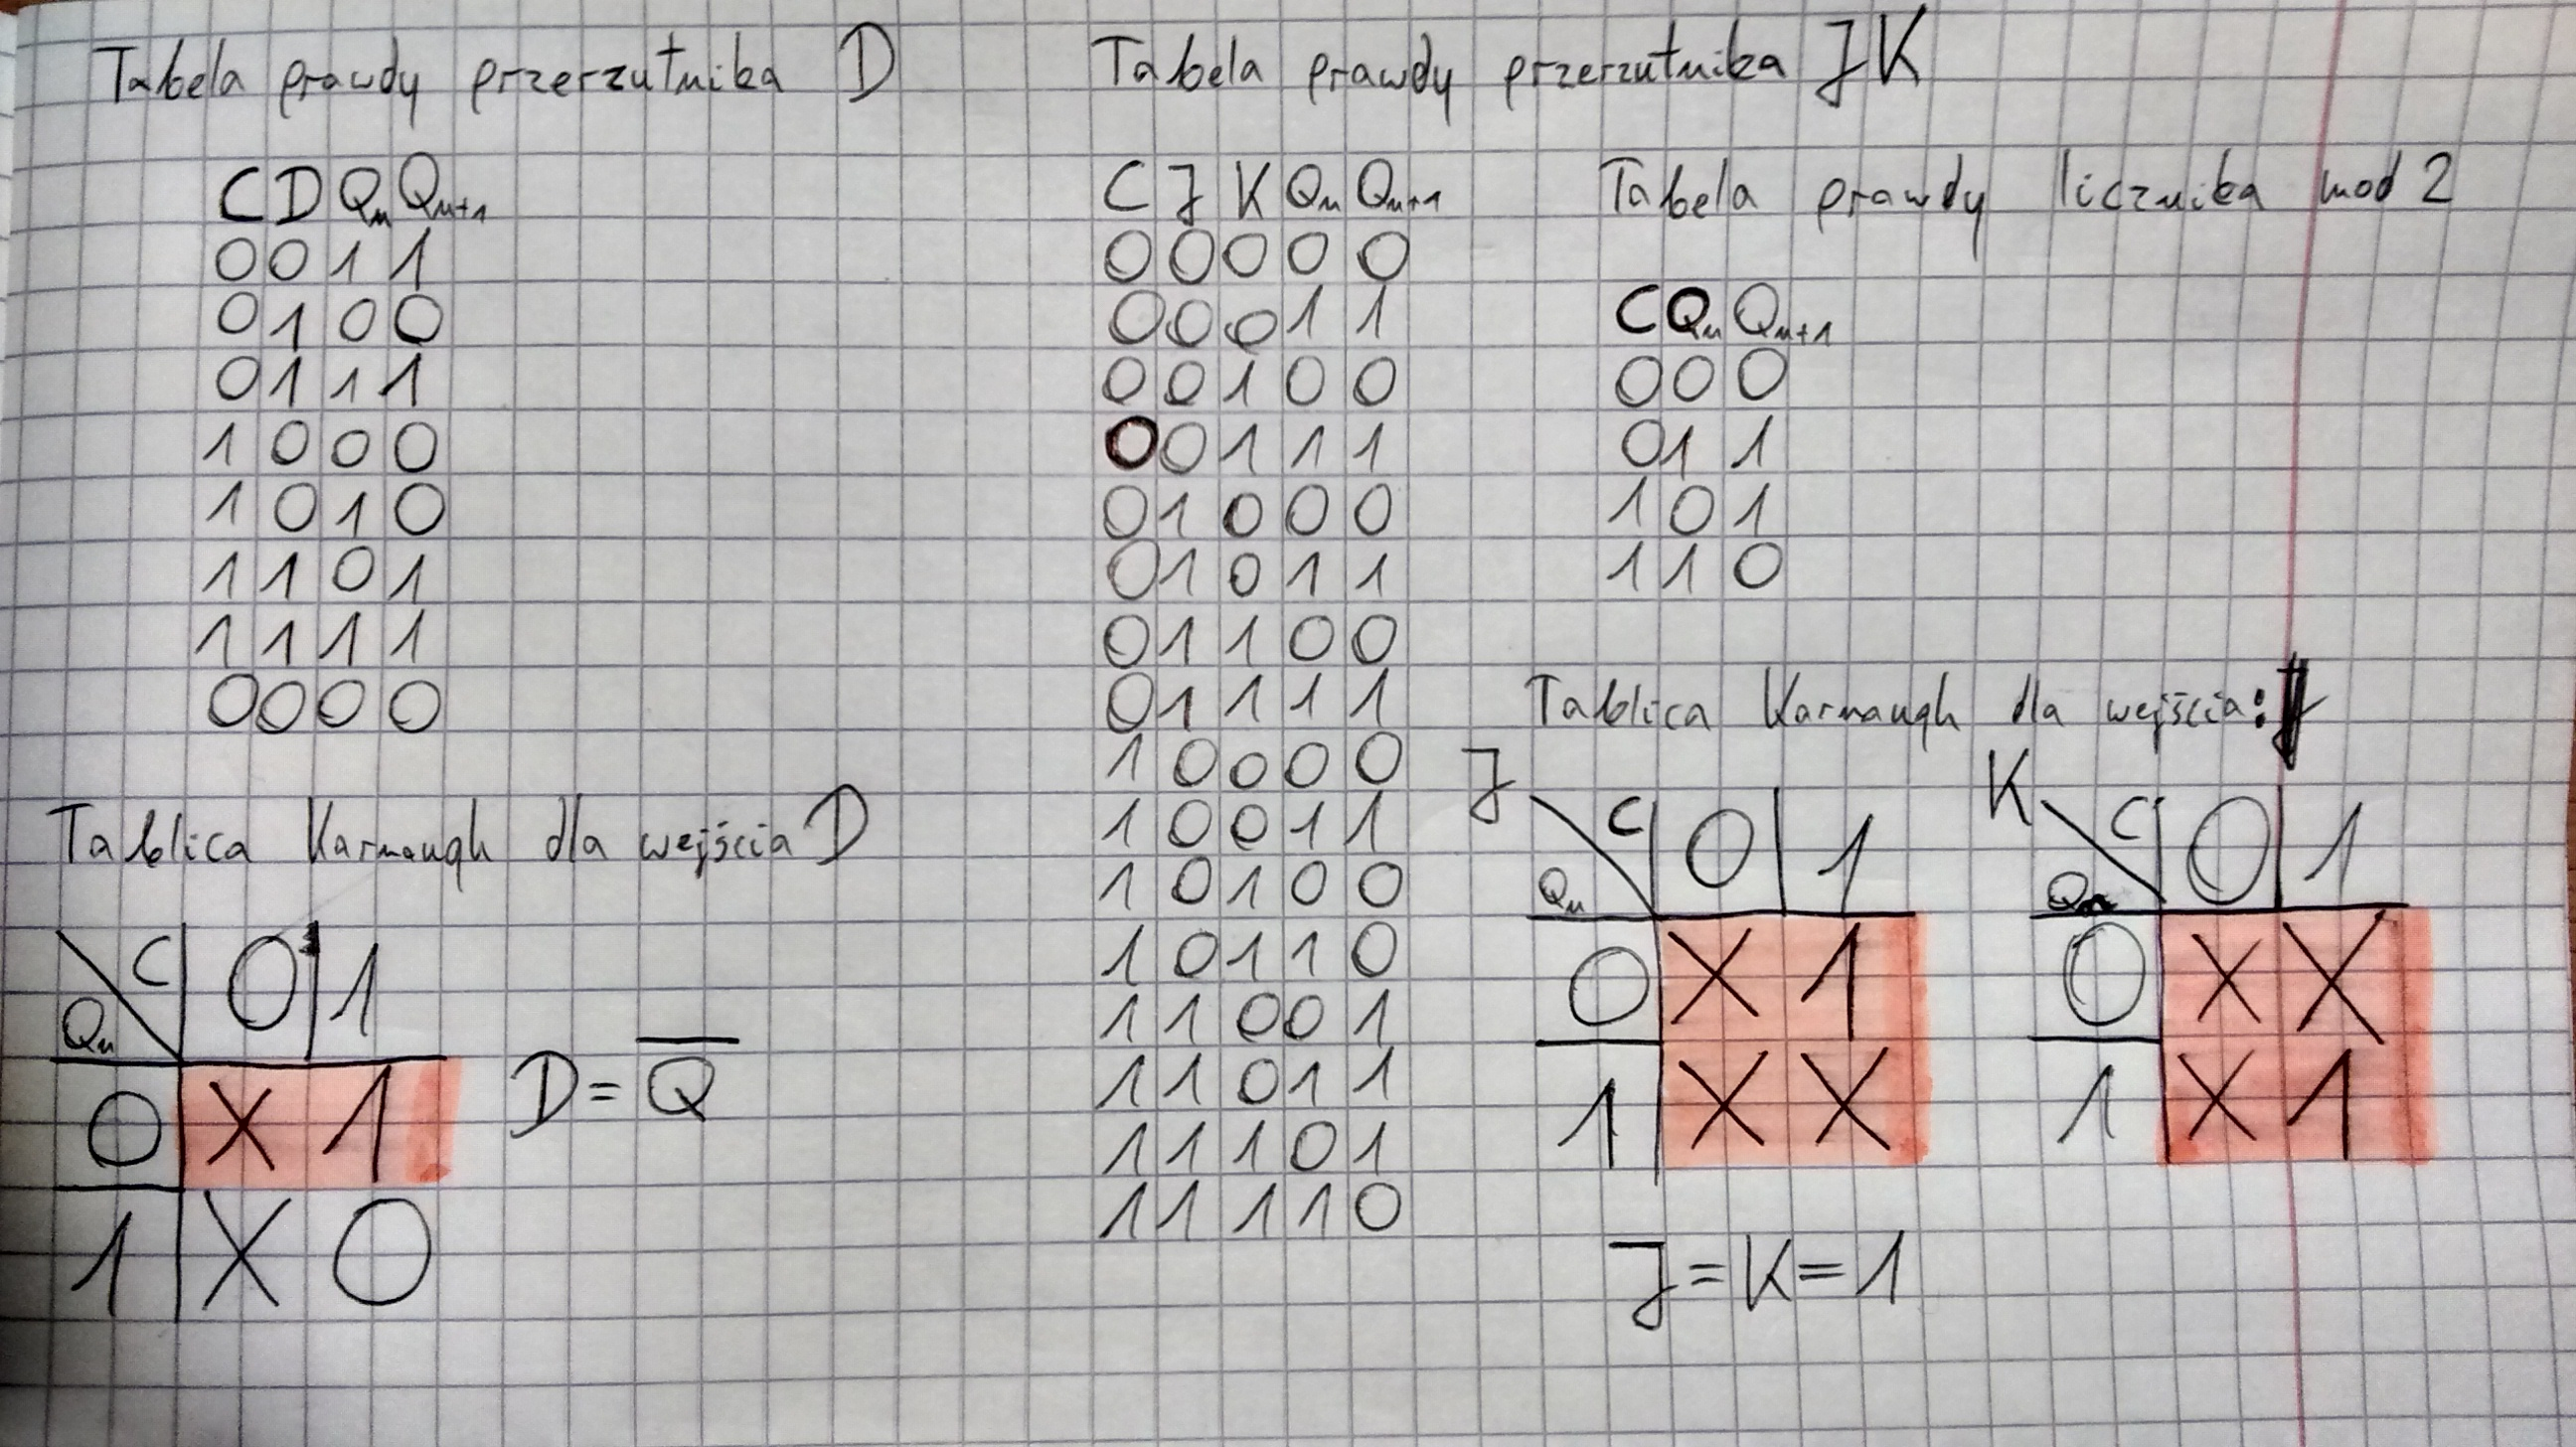
\includegraphics[width=\textwidth]{img/4a_tables}
\end{figure}

\newpage
Zbudowano odpowiadające im układy w Multisimie.
\begin{figure}[H]
\centering
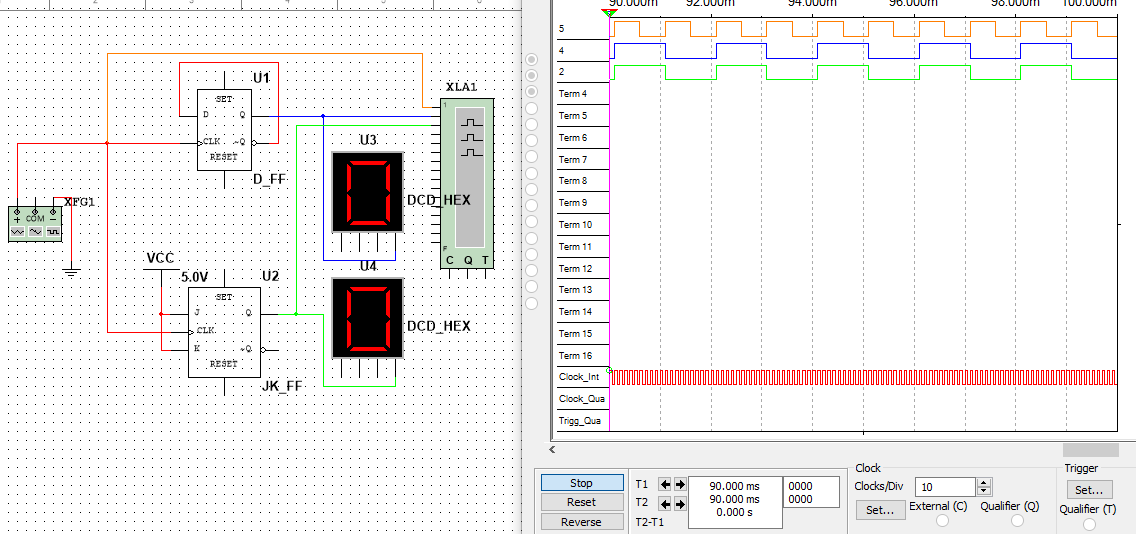
\includegraphics[width=\textwidth]{img/4a_circuit}
\end{figure}

Zaobserwowano prawidłowe działanie układów. Widzimy, że wyjście dwójki liczącej też jest zegarem, tyle że z okresem dwa razy dłuższym niż wejściowy, z czego skorzystamy przy budowie licznika asynchronicznego.


\section{Czterobitowy licznik asynchroniczny}
Przy budowie licznika czterobitowego skorzystałem z przerzutników T, których poznana wcześniej zasada działania wydała mi się optymalna do tego celu. Jeden przerzutnik odpowiada jednemu bitowi wyjścia. Korzystając z zaobserwowanego wcześniej faktu, że dwójka licząca daje sygnał zegarowy o okresie 2 razy dłuższym niż wejściowy, a każdy kolejny bit powinien przeskakiwać z 2 razy mniejszą częstotliwością niż poprzedni, aby uzyskać ten efekt, wystarczy połączyć wyjście każdego kolejnego przerzutnika z wejściem zegarowym kolejnego.

Na tej podstawie zbudowano układ w Multisimie.
\begin{figure}[H]
\centering
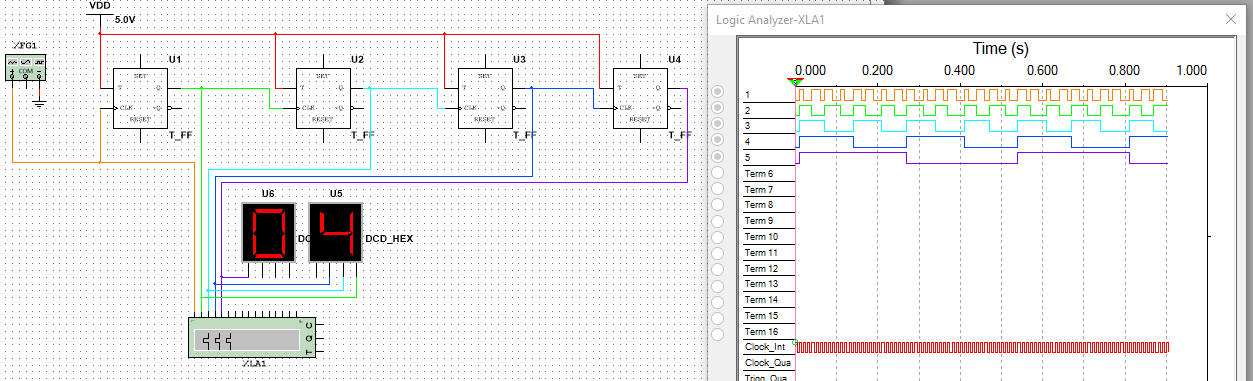
\includegraphics[width=\textwidth]{img/4b_circuit}
\end{figure}

Widzimy, że kolejne bity



\section{Synchroniczny licznik mod 8}

Liczniki synchroniczne rozwiązują problem liczników asynchronicznych - sygnał zegara jest podawany na każdy z przerzutników osobno, zatem redukuje się czas opóźnień.

Ponieważ licznik jest modulo 8, to wystarczy, by jego wyjście było 3-bitowe.

Rozważmy tabelę prawdy dla każdego z wyjść licznika:

\begin{figure}[H]
\centering
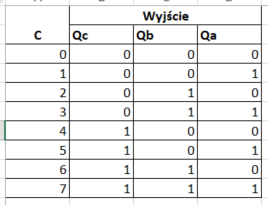
\includegraphics{img/4c_table}
\end{figure}

Na tej podstawie można stworzyć tabele Karnaugh'a dla funkcji logicznych sterujących przerzutnikami D.
Przypomnijmy, że wyjście przerzutnika D przyjmuje wartość sygnału podanego na wejście D, gdy na wejście zegarowe podany jest sygnał wysoki.
W poniższych tabelach przez Qc, Qb i Qa rozumiemy wartości tych wyjść przy poprzednim sygnale zegara:
 

\begin{figure}[H]
\centering
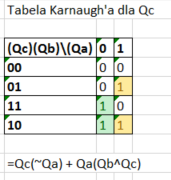
\includegraphics{img/4c_table_qc}
\end{figure}

\begin{figure}[H]
\centering
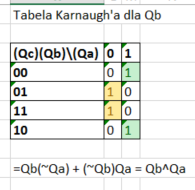
\includegraphics{img/4c_table_qb}
\end{figure}

\begin{figure}[H]
\centering
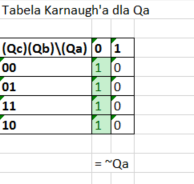
\includegraphics{img/4c_table_qa}
\end{figure}

Na podstawie uzyskanych funkcji logicznych zrealizowano następujący układ, w którym wejścia D przerzutników są sterowane uzyskanymi funkcjami:


\begin{figure}[H]
\centering
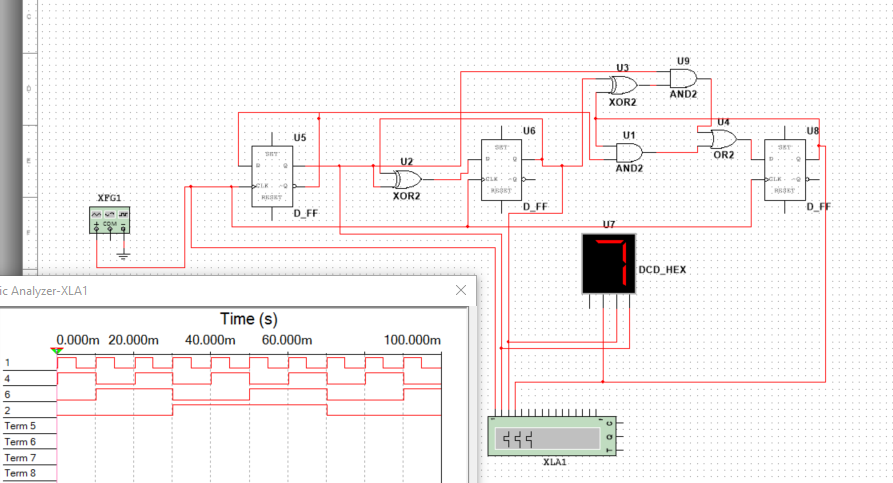
\includegraphics[width=\textwidth]{img/4c}
\end{figure}

\section{Synchroniczny licznik mod 6}
Mając synchroniczny licznik mod 8, zrealizowanie licznika mod 6 nie jest dużym wyzwaniem. Zgodnie z tabelą prawdy dla tego licznika:

\begin{figure}[H]
\centering
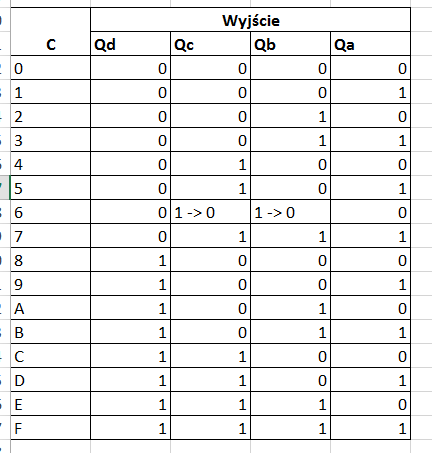
\includegraphics{img/4d_table}
\end{figure}

Wszystkie przerzutniki muszą zostać wyzerowane, gdy na wyjściach Qc i Qb pojawią się sygnały dodatnie. Aby to zrealizować, do schematu licznika modulo 8 dodano małą modyfikację - zerowanie przerzutników sygnałem z bramki AND łączącej Qc i Qb:

\begin{figure}[H]
\centering
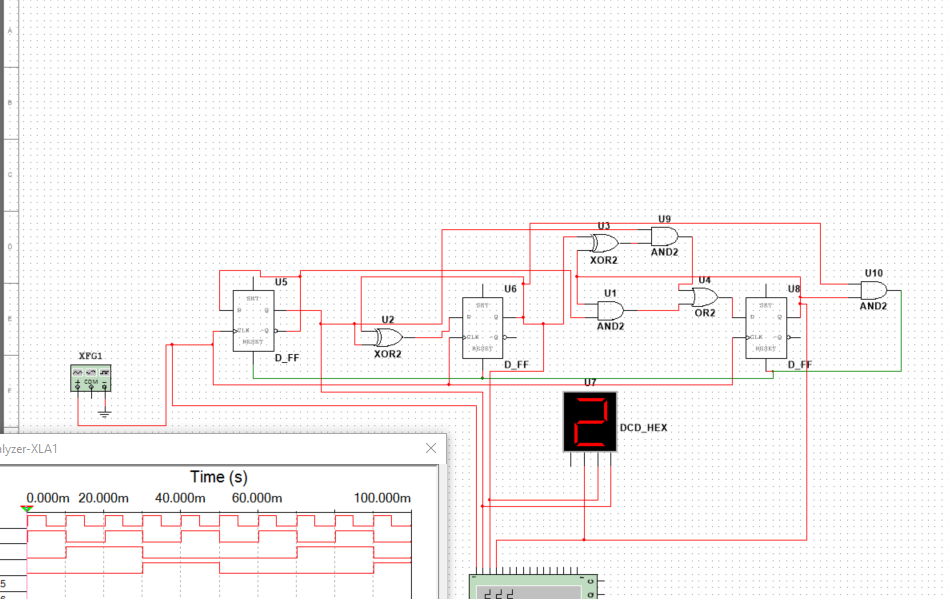
\includegraphics[width=\textwidth]{img/4d}
\end{figure}






\end{document}
